\chapter{Migration}
\label{sec:migration}

Resources allocation to jobs is a difficult task to execute optimally and often depends on a plethora of different factors. Most job schedulers are conceived to schedule jobs and allocate resources to them upfront, with only limited abilities to intervene once a job entered the running state.

Process migration, or, in this specific case, \gls{vm} migration, allows to dynamically adjust resource allocation and job scheduling as new information becomes available even if a job was already started. This runtime adjustment is applied to the system by moving jobs from one resource to another as necessity arises.

The \autoref{fig:migration-process} provides an example of the concept of \gls{vm} migration applied to the scheduling of virtual clusters on resources managed by the \emph{Physical cluster provisioner} described in \autoref{sec:remotevirt}. In this scenario, a virtual clusters is resized through \glspl{vm} migration in order to take account for an additional job submitted to the system.

In the illustration, each square represents a physical node, each circle a virtual machine (using different colors for \glspl{vm} belonging to different virtual clusters) and each shaded rectangle a virtual cluster.

\begin{figure}[h]
	\subfloat[Low load operation]{
		\label{fig:low-load}
		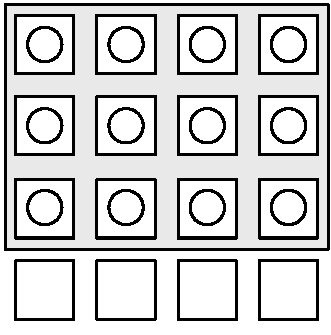
\includegraphics[width=.23\textwidth]{figures/statement/low-load}
	}
	\hfill
	\subfloat[Migration]{
		\label{fig:migration}
		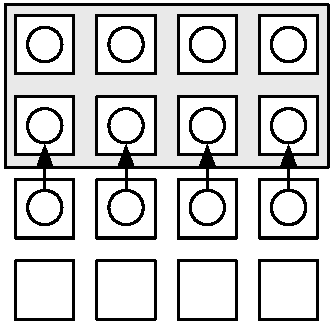
\includegraphics[width=.23\textwidth]{figures/statement/migration}
	}
	\hfill
	\subfloat[High load operation]{
		\label{fig:high-load}
		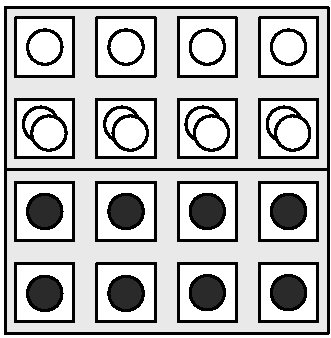
\includegraphics[width=.23\textwidth]{figures/statement/high-load}
	}
	\hfill
	\subfloat[Restoration]{
		\label{fig:restoration}
		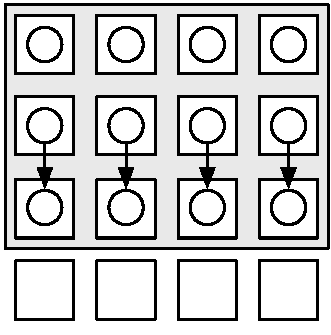
\includegraphics[width=.23\textwidth]{figures/statement/migration-back}
	}
	\caption{Example of virtual cluster resizing through VMs migration.}
	\label{fig:migration-process}
\end{figure}

The step \ref{fig:low-load} illustrates the state of the different nodes in a stable situation with one virtual cluster consisting of twelve virtual machines. The step \ref{fig:migration} shows how the system reacts as soon as a new virtual cluster request is submitted to the system: some \glspl{vm} are migrated to already busy nodes of the same cluster (oversubscription) to free up resources for the new virtual cluster. The freed up resources are then allocated to the new virtual cluster as shown in step \ref{fig:high-load}. The step \ref{fig:restoration} shows how an optimal resource usage is restored once one of the virtual clusters is released and more resources become available again.

Basic support for this scheduling and allocation enhancements is provided by the current \gls{vurm} implementation. In order to be able to account for different allocation, scheduling and migration techniques and algorithms, the different involved components are completely pluggable and can easily be substituted individually.

In order to further describe the different components and the implemented techniques and algorithms, the present chapter is structured in the following sections:

\begin{itemize}
	\item Section~\ref{sec:migration-framework} introduces the migration framework put in place to support alternate pluggable resource allocators and migration schedulers by describing the involved data structures and the responsibilities of the different components;
	\item Section~\ref{sec:allocation-strategy} describes the resources allocation strategy implemented in the default resource allocator shipped with the \gls{vurm} implementation;
	\item Similarly as done for the previous section, section~\ref{sec:scheduling-strategy} describes the default migration scheduling strategy and offers insights over the optimal solution;
	\item Section~\ref{sec:migration-techniques} introduces the different approaches to \gls{vm} migration and describes the implemented solution as well as the issues encountered with the alternate techniques;
	\item To conclude, section~\ref{sec:migration-improvements} resumes some of the possible improvements which the current \gls{vurm} version could take advantage of but which weren't implemented due to different constraints.
\end{itemize}


\section{Migration framework}
\label{sec:migration-framework}

Different job types, different execution contexts or different available resources are all factors which can led to chose one given resource allocation or job scheduling algorithm over another. A solution which works equally well in every case does not exists and as such, users and system administrators, want to be able to adapt the strategy to the current situation.

In order to provide support for configurable and pluggable schedulers and allocators, a simple framework was put in place as part of the \emph{Physical cluster provisioner} architecture. This section describes the different intervening entities, their responsibility and the data structures exchanged between them.

The \autoref{fig:migration-framework} illustrates the class diagram of the migration framework. Most of the represented classes were taken from the physical cluster provisioner class diagram (\autoref{fig:remotevirt-arch} on page \pageref{fig:remotevirt-arch}); newly added classes, attributes and operations are highlighted using a lighter background color.

\begin{figure}
	\centering
	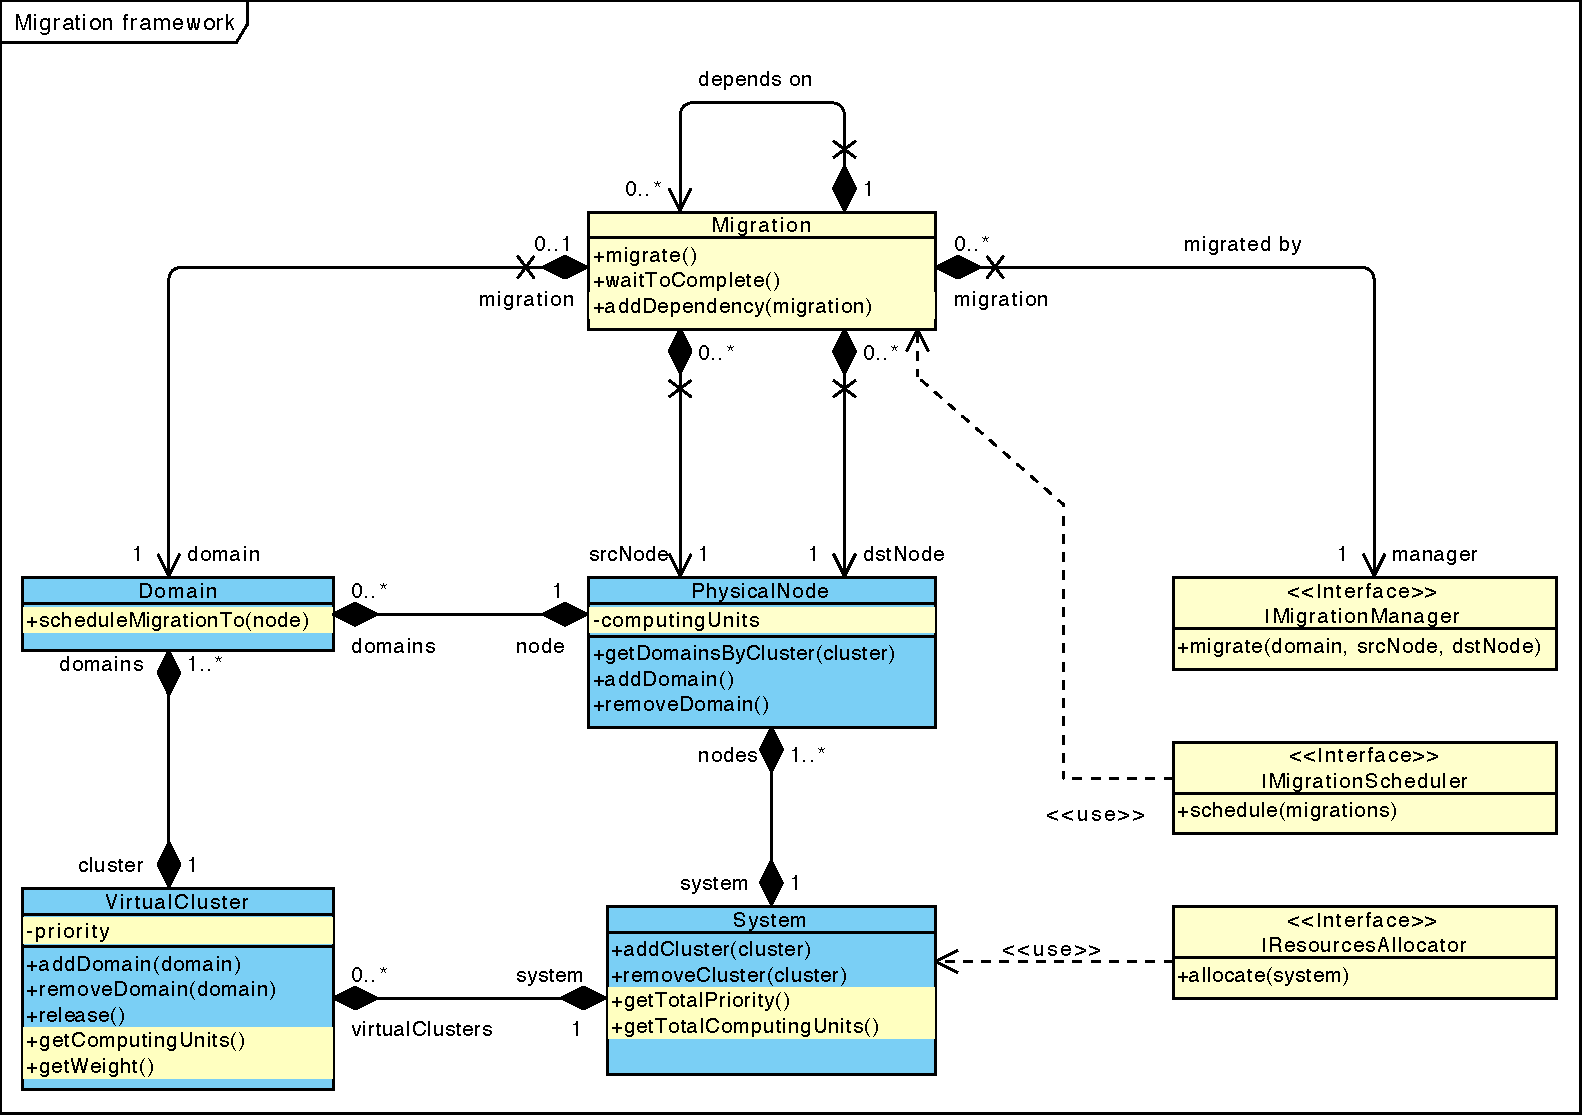
\includegraphics[width=1\textwidth]{figures/migration-framework}
	\caption{Migration framework components}
	\label{fig:migration-framework}
\end{figure}

As shown in the class diagram, three new interfaces were added to the architecture. Each of these interfaces is responsible for a different task in the whole migration operation. The newly added members to the already existing classes and the \texttt{Migration} class were added to help the three interface realizations make the right decisions and communicate them back to the resource provisioner for it to carry them out.


\subsection{Node and cluster weighting}

The current version of the \gls{vurm} \texttt{remotevirt} provisioner allows to assign a fixed \gls{cu} value to each physical node $PN$ in the system. A computing unit is simply a relative value comparing a node to other nodes in the system: if Node A has a $\gls{cu}$ value of 1 while Node B has a value of 2, then Node B is assumed to be twice as powerful as Node A. Note that these values do not express any metrics about the absolute computing power of either node but only the relationship between them.

The total power of the system $CU_{sys}$ is defined as the sum of all computing units of each node in the system itself (\autoref{eq:cusys}). It is possible to access these values by reading the value contained in the \texttt{computingUnits} property of a \texttt{PhysicalNode} instance or by calling the \texttt{getTotalComputingUnits} method on the \texttt{System} instance.

\begin{equation}
	\label{eq:cusys}
	CU_{sys} = \sum_{i=0}^n CU_{PN_i}
\end{equation}

Similarly as done for physical nodes, it is possible to assign a fixed priority $P$ to a virtual cluster $VC$ at creation time. As for the \glspl{cu}, the priority is also a value relative to other clusters in the system: if Virtual Cluster A and Virtual Cluster B have the same priority, they will both have access to the same amount of computing power. The weight of a virtual cluster  $W_{VC}$ is defined as the ratio between the priority of the cluster and the sum of the priorities of all the clusters in the system (\autoref{eq:weight}); this value indicates the fraction of computing power the virtual cluster has right to.

\begin{equation}
	\label{eq:weight}
	W_{VC_i} = \frac{P_{VC_i}}{\sum_{i=0}^n P_{VC_i}}
\end{equation}

The exact amount of computing power assigned to a cluster $CU_{VC}$ is easily calculated by multiplying the weight with the total computing power of the system (\autoref{eq:cuvc}).

\begin{equation}
	\label{eq:cuvc}
	CU_{VC_i} = W_{VC_i} \cdot CU_{sys}
\end{equation}

Methods to calculate all those values are provided by the \gls{vurm} implementation itself and are not needed to be carried out by the resources allocators. The next subsection illustrates how these values and the provided data structures are used by the three interface realizations to effectively reassign resources to different \glspl{vm}, schedule migrations in the optimal way and apply a given migration technique.


\subsection{Allocators, schedulers and migration managers}

The class diagram in the \autoref{fig:migration-framework} adds three new interfaces to the physical cluster provisioner architecture: the \texttt{IResourceAllocator} realization is in charge to decide which \glspl{vm} have to be migrated to which physical node, the \texttt{IMigrationScheduler} realization schedules migrations by defining dependencies between them in order to optimize the execution time and limit resources usage, and the \texttt{IMigrationManager} realization is responsible to actually carry out each single migration. Each one of these three interfaces have to be implemented by one or more objects and passed to the \texttt{remotevirt} provisioner at creation time.

The interactions between the provisioner and these three components of the migration framework is illustrated in the sequence diagram in \autoref{fig:migration-sequence} on page \pageref{fig:migration-sequence}. Each one of the intervening components is further described in the following paragraphs.

\begin{figure}[h]
	\centering
	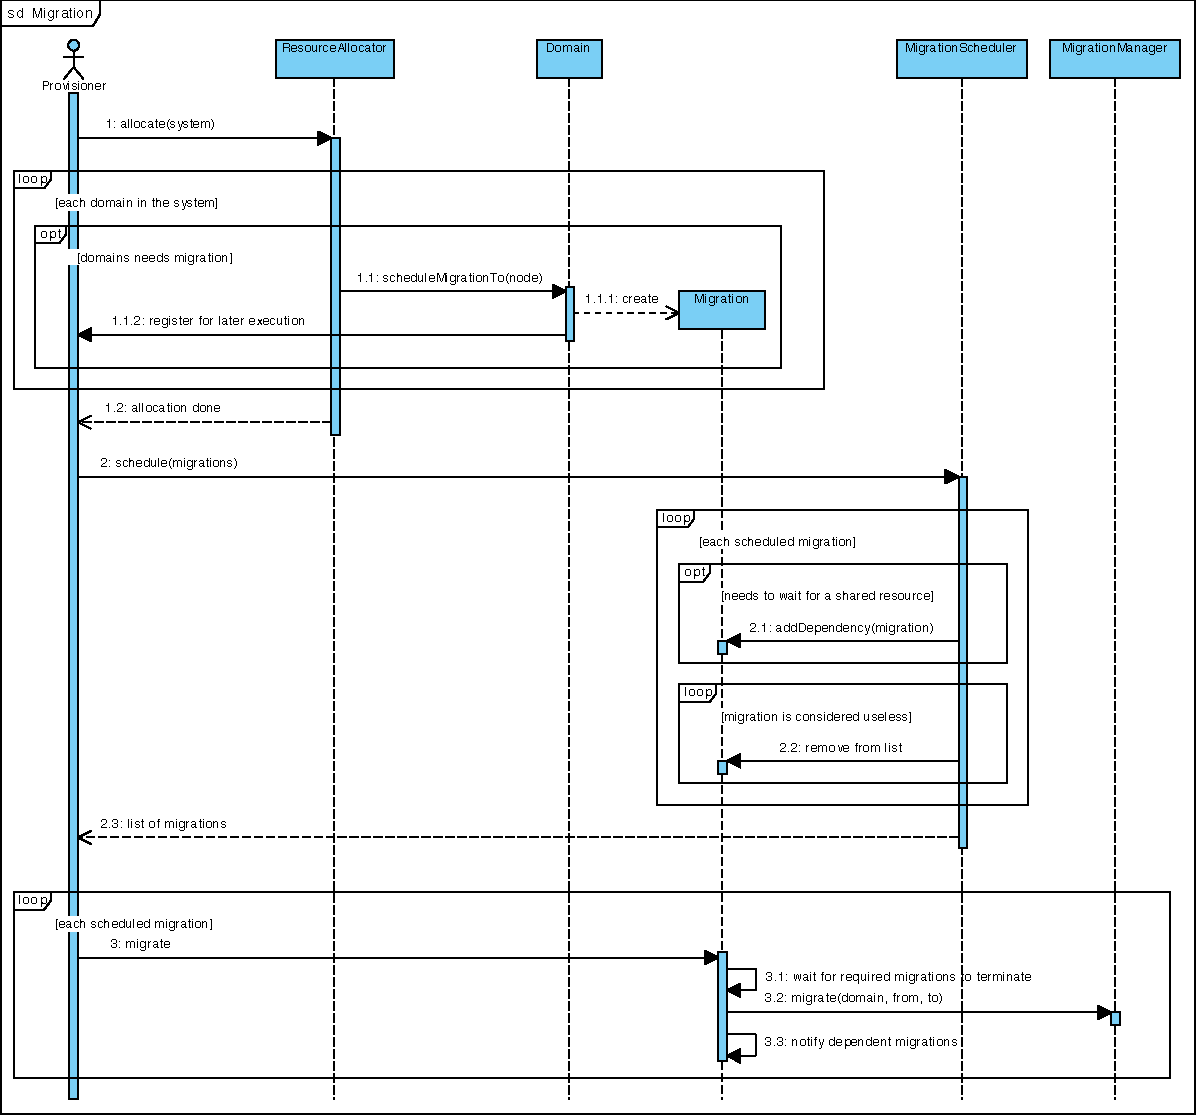
\includegraphics[width=1\textwidth]{figures/migration-sequence}
	\caption{Collaboration between the different components of the migration framework}
	\label{fig:migration-sequence}
\end{figure}

\subsubsection{Resource allocator}

The \texttt{allocate} method of the configured \emph{resource allocator} instance is invoked when a resource reallocation is deemed necessary by the provisioner (refer to the next subsection for more information about the exact migration triggering strategy).

The method takes the current \texttt{System} instance as its only argument and returns nothing. It can reallocate resources by migrating virtual machines from one physical node to another. To do so, the implemented allocation algorithm has to call the \texttt{scheduleMigrationTo} method of the \texttt{Domain} instance it wants to migrate.

Scheduled migrations are not carried out immediately but deferred for later execution, in order to allow for the migration scheduler to optimize their concurrent execution.

\subsubsection{Migration scheduler}

Once the resource allocator has decided which virtual machines need to be moved to a different node and the respective migrations have been scheduled, the \texttt{schedule} method of the \emph{migration scheduler} instance is invoked. 

This method receives a list of \texttt{Migration} instances as its only argument and returns a similar data structure. Its task is to define dependencies between migrations in order to optimize the resource usage due to their concurrent execution.

To add a new dependency, the implemented algorithm has to call the \texttt{addDependency} method of the \emph{dependent} \texttt{Migration} instance. All the migration instances still present in the returned list will be executed by respecting the established dependencies, it is thus possible to prevent a migration from happening simply by not inserting it in the returned list.

\subsubsection{Migration manager}

Different migration techniques (e.g. offline, iterative precopy, demand migration,…) are available to move a virtual machine from a physical node to another.\footnote{A deeper analysis of the different techniques is exposed in \autoref{sec:migration-techniques}.} It is the responsibility of the \emph{migration manager} to decide which migration technique to apply for each given migration.

Each migration contained in the list returned from the \texttt{schedule} invocation is triggered by the provisioner. When told to start, the \texttt{Migration} instances wait for all migrations they depend on to finish and subsequently defer their execution to the responsible \texttt{MigrationManager} instance by calling its \texttt{migrate} method. Lastly, once the migration is terminated, each migration instance notifies the dependent migrations that they can now start.


\subsection{Migration triggering}

The whole resource allocation, migration scheduling and actual migration execution is triggered by the provisioner in exactly three cases:

\begin{enumerate}
	\item \emph{Each time a new virtual cluster is created.} This triggering method waits for a given (configurable) stabilization period to be over before effectively starting the process. Thanks to the stabilization interval, if two virtual cluster creation or releasing requests are received in a short time interval, only one scheduling will take place;
	\item \emph{Each time a virtual cluster is released.} Similarly as done for the creation trigger, the stabilization interval is applied in this case too. The stabilization interval is reset in both cases, regardless of the type of request (creation or release) which is received;
	\item \emph{At regular intervals.} If no clusters are created or released, a resources reallocation is triggered at a regular and configurable interval. Interval triggers are momentarily suspended when the triggering system is waiting for the stabilization period to be over.
\end{enumerate}



\section{Allocation strategy}
\label{sec:allocation-strategy}

The \texttt{remotevirt} provisioner ships with a default resource allocator implementation called \texttt{SimpleResourceAllocator}. This section aims to describe the implemented resource allocation algorithm.

The \texttt{SimpleResourceAllocator} allocates resources on a static system view basis. This means that each time a new resource allocation request is made, the algorithm only cares about the current system state and does not take into account previous states. Additionally, the algorithm bases its decision only on the cluster priorities and the \glspl{cu} assigned to the physical nodes.

The implemented algorithm can be divided in four different steps; each one of these steps is further described in the remaining part of this section.

\subsection{Cluster weighing}
\label{sec:cluster-weighing}

This step takes care of assigning an integer computing unit value to each cluster while accounting for rounding errors. An integer value is needed because in this simple allocator version, nodes are not shared between clusters (which means that it is not possible to allocate only a fraction of a node to a virtual cluster). The algorithm pseudocode to round the value calculated using the \autoref{eq:cuvc} is reported in \autoref{lst:curounding}.
	
\lstset{language=python,caption=CU rounding algorithm,label=lst:curounding}
\begin{lstlisting}
# Create a list of computing units and clusters tuples
computingUnits = [(c.getComputingUnits(), c) for c in clusters]

# Calculate the quotient and the remainder of each computing unit
computingUnits = [(cu % 1, int(cu), c) for cu, c in computingUnits]

# Calculate the remainder of the truncated computing units sum
remainder = sum([rem for (rem, _, _) in computingUnits])

# Sort computing units in reverse order by remainder and create an iterator
adjustements = iter(sorted(computingUnits, reverse=True))

# While there is some remainder left, increment the next cluster with
# the largest remainder
while remainder:
	next(adjustements)[1] += 1
	remainder -= 1
\end{lstlisting}

The \autoref{tab:rounding-algo} provides an example of the application of the described algorithm to a system containing six virtual clusters. The exact value, the rounded value and the algorithm value are calculated for two different scenarios: once for a system with a total $CU$ of 10 and a second time for the same system but with a $CU$ value of 15.

\begin{table}
\begin{tabularx}{\textwidth}{ r R X | C C C | C C C }

\toprule

% Headers
\multirow{2}{*}{$i$} & \multirow{2}{*}{$PC_{VC_i}$} & \multirow{2}{*}{$W_{VC_i}$} &
\multicolumn{3}{c|}{$CU_{VC_i}$ with $CU_{sys}=10$} &
\multicolumn{3}{c}{$CU_{VC_i}$ with $CU_{sys}=15$} \\
\cline{4-9}
& & & Exact & Rounded & Algo & Exact & Rounded & Algo \\
\hline

% Contents
0 & 24  & 0.08 & 0.8 & 1 & 1 & 1.2 & 1 & 1 \\
1 & 6   & 0.02 & 0.2 & 0 & 0 & 0.3 & 0 & 0 \\
2 & 84  & 0.28 & 2.8 & 3 & 3 & 4.2 & 4 & 4 \\
3 & 108 & 0.36 & 3.6 & 4 & 4 & 5.4 & 5 & 6 \\
4 & 48  & 0.16 & 1.6 & 2 & 1 & 2.4 & 2 & 2 \\
5 & 30  & 0.10 & 1.0 & 1 & 1 & 1.5 & 2 & 2 \\

% Footer
\hline
\textbf{Totals} & 300 & 1.00 & 10 & 11 & 10 & 15 & 14 & 15 \\
\bottomrule
\end{tabularx}

\caption{Rounding algorithm example with two different $CU_{sys}$ values}
\label{tab:rounding-algo}
\end{table}


\subsection{Nodes to cluster allocation}

Once that each cluster has an integer computing unit value attached to it, the algorithm goes on by assigning a set of nodes to each virtual cluster in order to fulfill its computing power requirements.

The implemented algorithm assigns nodes to clusters starting with the cluster with the highest computing unit assigned to it and then proceeding in descending order. Firstly, the most powerful available node is allocated to the current cluster\footnote{This prevents large nodes (i.e. exceeding the requirements of the most demanding cluster) to be left unused.} and then the algorithm iterates over all available nodes in descending computing power order and assigns them to the cluster as long as the cluster computing power is not exceeded.

The \autoref{lst:nodetovc} illustrates a simplified version of the implemented algorithm. Note that the allocated computing units (\texttt{currentPower}) is also returned as it can differ from the threshold value (\texttt{assignedComputingUnits}).

\lstset{language=python,caption=Nodes to virtual cluster allocation,label=lst:nodetovc}
\begin{lstlisting}
# Initialize data structure and variables
clusterNodes = [availableNodes.pop(0)]
currentPower = clusterNodes[0].computingUnits

# If the power is not already exeeded
if currentPower < assignedComputingUnits:
	for n in availableNodes:
		# If adding this node to the cluster does not exceed the assigned CUs
		if currentPower + n.computingUnits < assignedComputingUnits:
			availableNodes.remove(n)  # Move the node...
			clusterNodes.append(n)    # ...to the cluster nodes list
			currentPower += n.computingUnits

# Return the real computing power of the virtual cluster and the assigned nodes
return currentPower, clusterNodes
\end{lstlisting}

\subsection{VMs to nodes allocation}

This third step of the algorithm provides to assign a certain number of \glspl{vm} to each node in the cluster basing on the computing units of the node, the total computing units assigned to the virtual cluster and the number of \glspl{vm} running inside it.

The exact number of virtual machines $VM_{PN_i}$ assigned to a node $i$ of the virtual cluster $j$ is calculated as show in \autoref{eq:vmtonode}. Once the exact value is calculated for each physical node of the virtual cluster, the same rounding algorithm as used for the \emph{\nameref{sec:cluster-weighing}} step is applied.

\begin{equation}
	\label{eq:vmtonode}
	VM_{PN_i} = VM_{VC_j} \cdot \frac{CU_{PN_i}}{CU_{VC_j}}
\end{equation}

\subsection{VMs migration}

The remaining part of the resources allocation algorithm is responsible to decide which virtual machine has to be migrated to which physical node. This part has been divided into two distinct sets of migrations.

The first migrations set is responsible to migrate all virtual machines currently running on nodes reassigned to other virtual clusters to a free node of the virtual cluster to which the virtual machine belongs to. This first iteration is reported in the \autoref{lst:extmigration}.

\lstset{language=python,caption=VMs migration from external nodes,label=lst:extmigration}
\begin{lstlisting}
# nodesVMCount is a list of (node, number of vm) tuples
idleNodesIter = iter(nodesVMCount)

# Initialize the variables
node, maxCount = next(idleNodesIter)

for domain in cluster.domains:
	# If the virtual machine is running on an external node
	if domain.physicalNode not in clusterNodes:
		# If the current node is already completely subscribed
		while len(node.domainsByCluster(cluster)) >= maxCount:
			# Find the next node which has a VM slot available
			node, maxCount = next(idleNodesIter)
		# Migrate the VM to the chosen node
		domain.scheduleMigrationTo(node)
\end{lstlisting}

The second migration set is responsible to migrate \glspl{vm} between different nodes of the same virtual cluster in order to reach the correct number of assigned virtual machines running on each node. This is necessary because depending on the set of nodes assigned to a cluster, a given node could be running more virtual machines than the allocated number.

\lstset{language=python,caption=Leveling node usage inside a virtual cluster,label=lst:insidemigration}
\begin{lstlisting}
# The filterByLoad function creates three separate lists from the given 
# nodesVMCount variable. A list of nodes with available slots, a list of 
# already fully allocated nodes, and a list of oversubscribed nodes.
idle, allocated, oversubscribed = filterByLoad(nodesVMCount, cluster)

for node, count in oversubscribed:
	# Get an iterator over each domain belonging to cluster running on the 
	# oversubscribed node
	domains = iter(node.domainsByCluster(cluster))
	
	for i in range(count):
		# For each domain exceeding the node capacity
		domain = next(domains)
		
		if not idle[0][1]:
			# Discard the current idle node if in the meantime it has 
			# reached its capacity
			idle.pop(0)

		# Update the number of running domains
		idle[0][1] -= 1
		# Migrate the domain to the idle node
		domain.scheduleMigrationTo(idle[0][0])
\end{lstlisting}

Once the second set of migrations was scheduled too, the resource allocator can return the control to the provisioner and wait for the next triggering to take place (message 1.2 in the sequence diagram on page \pageref{fig:migration-sequence}).



\section{Scheduling strategy}
\label{sec:scheduling-strategy}

\gls{vm} migration is an heavy task in terms of bandwidth and, depending on the used migration strategy, in terms of \glstext{cpu} usage. Running a multitude of simultaneous migrations between a common set of physical nodes can thus reduce the overall system responsiveness and saturate the network bandwidth, as well as lengthen the migration time and thus the downtime of the single \glspl{vm}.

To obviate to this problem, and to allow for different scheduling strategies to be put in place, the \texttt{remotevirt} provisioner supports a special component called \emph{migration scheduler}. The responsibility of this component is to schedule migrations by establishing different dependency links between the single migration tasks in order to keep resources usage under a certain threshold while optimizing the maximum number of concurrent migrations.

The default implementation shipped with the physical cluster provisioner is a simple \emph{noop} scheduler which lets all migrations execute concurrently. A more optimized solution was not implemented due to time constraints, but the problem was analyzed on a theoretical level and formulated in terms of a graph coloring problem. This section aims to explain the theoretical basis behind the optimal solution and provides the simple greedy algorithm for a possible future implementation.

The problem statement for which a solution is sought is formulated in the following way: \emph{find the optimal scheduling to execute all migrations using the minimum number of steps in such way that no migration involving one or more common nodes is carried out during the same step.}

By representing the migrations as edges connecting vertices (i.e. the physical nodes) of an undirected\footnote{The migration direction is not relevant for the problem formulation as the resource usage is assumed to be the same on both ends of the migration.} graph, the previous formulation can be applied to the more general problem of edge coloring. In graph theory, an edge coloring of a graph is an assignment of “colors” to the edges of the graph so that no two adjacent edges have the same color.

The \autoref{tab:migration1-table} lists the migrations used for the examples throughout this section. Similarly, the \autoref{fig:migration1-graph} represents the same migration set using an undirected graph.

\begin{minipage}{0.45\textwidth}
	\begin{flushleft}
		\begin{table}[H]
		\begin{tabularx}{\textwidth}{ C C C }

		\toprule
		% Headers
		Domain & Source~Node &  Dest.~Node \\
		\hline

		% Contents
		0 & A & E \\
		1 & A & D \\
		2 & C & B \\
		3 & B & D \\
		4 & D & A \\
		5 & A & C \\
		\bottomrule
		\end{tabularx}

		\caption{Migrations in tabular format}
		\label{tab:migration1-table}
		\end{table}
	\end{flushleft}
\end{minipage}
\hfill
\begin{minipage}{0.45\textwidth}
	\begin{flushright}
		\begin{figure}[H]
			\centering
			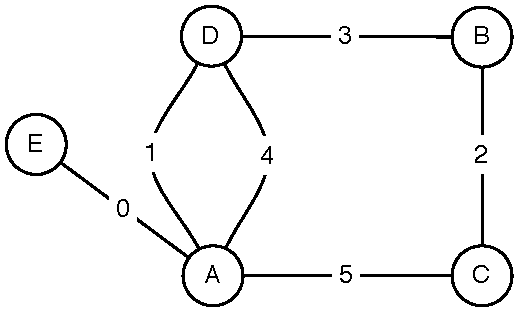
\includegraphics[width=1\textwidth]{figures/migration-example-1}
			\vspace*{-1.5mm}
			\caption{Graphical representation}
			\label{fig:migration1-graph}
		\end{figure}
	\end{flushright}
\end{minipage}

Once the edges are colored, it is possible to execute migrations concurrently as long as they share the same color. The subfigure~\ref{fig:migration-coloring} shows one of the possible (optimal) coloring solution and the subfigure~\ref{fig:migration-dependencies} one of the possible migration scheduling resulting from this coloring solution represented as a \gls{dag}.


\begin{figure}[h]
	\subfloat[One possible edge coloring solution]{
		\label{fig:migration-coloring}
		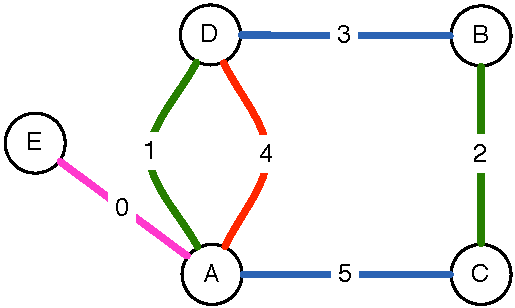
\includegraphics[width=.45\textwidth]{figures/migration-example-1-color}
	}
	\hfill
	\subfloat[Chosen migration scheduling]{
		\label{fig:migration-dependencies}
		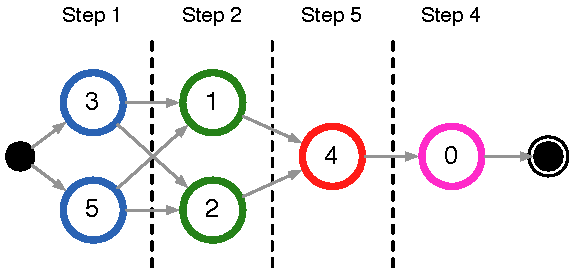
\includegraphics[width=.45\textwidth]{figures/migration-example-1-schedule}
	}
	\caption{Edge coloring and the respective migration scheduling.}
	\label{fig:migration-process-2}
\end{figure}

By Vizing's theorem \cite{vizing}, the number of colors needed to edge color a simple graph is either its maximum degree $\Delta$ or $\Delta+1$. In our case, the graph can be a multigraph because multiple migrations can occur between the same two nodes and thus the number of colors may be as large as $3\Delta/2$.

There are polynomial time algorithms that construct optimal colorings of bipartite graphs, and colorings of non-bipartite simple graphs that use at most $\Delta+1$ colors \cite{bipartite}; however, the general problem of finding an optimal edge coloring is NP-complete and the fastest known algorithms for it take exponential time.

A good approximation is offered by the greedy coloring algorithm applied to the graph vertex coloring problem. The graph vertex coloring problem is the same as the edge coloring problem but applied to adjacent vertices instead. As the edge chromatic number of a graph $G$ is equal to the vertex chromatic number of its line graph $L(G)$, it is possible to apply this algorithm to the edge coloring problem as well.

Greedy coloring exploits a greedy algorithm to color the vertices of a graph that considers the vertices in sequence and assigns each vertex its first available color. Greedy colorings do not in general use the minimum number of colors possible and can use as much as $2\Delta - 1$ colors (which may be nearly twice as many number of colors as is necessary); however the algorithm exposes a time complexity of $O(\Delta^2 + log^{*}n)$ for every $n$-vertex graph \cite{greedy-complexity} and it has the advantage that it may be used in an online algorithm setting in which the input graph is not known in advance. In this setting, its competitive ratio is two, and this is optimal for every online algorithm \cite{greedy}.

More complex formulations of the migration problem can also be made. It could be interesting to be able to configure a maximum number of concurrent migrations occurring on each node instead of hard limiting this value to one. This enhancement would allow to better exploit the available resources as the time ${\Delta}t_{n-concurrent}$ taken for $n$ concurrent migrations between the same nodes is less than $n$ times the duration of a single migration ${\Delta}t_{single}$ (\autoref{eq:concurrent-migrations}).

\begin{equation}
	{\Delta}t_{n-concurrent} < n \cdot {\Delta}t_{single}
	\label{eq:concurrent-migrations}
\end{equation}

Empirical measures have shown that fully concurrent migration setups can achieve as much as $20\%$ speedup over single-scheduled migrations by trading off for a complete network saturation and very high \glstext{cpu} loads. A configurable value for the maximum number of concurrent migrations would allow to adjust the \emph{speed/load} tradeoff to the runtime environment.


\section{Migration techniques}
\label{sec:migration-techniques}

It is not yet possible to migrate a virtual machine from one physical node to another without any service downtime. Different migration techniques exist thus to try to minimize the \gls{vm} downtime, often while trading off for a longer migration time.

Service downtime is defined as the interval between the instant at which the \gls{vm} is stopped on the source host and the instant at which it is completely resumed on the destination host. Migration time is defined as the interval between the reception of the migration request and the instant at which the source host is no more needed for the migrated \gls{vm} to work correctly on the destination host

This section aims to introduce some of the most important categories of \gls{vm} migration techniques and illustrate the method adopted by the \gls{vurm} \texttt{remotevirt} provisioner.

The most basic migration technique is called \emph{offline migration}. Offline migration consists in completely suspending the \gls{vm} on reception of the migration request, copying the whole state over the network to the destination host, and resuming the \gls{vm} execution there. Offline migration accounts for the smallest migration time and the highest service downtime (the two intervals are approximately the same).

All other migration techniques are a subset of live migration. These migration implementations seek to minimize downtime by accepting a longer overall migration time. Usually these algorithms generalize memory transfer into three phases \cite{clark} and are implemented by exploiting one or two of the three:

\begin{itemize}
	\item \textbf{Push phase} The source \gls{vm} continues to run while certain pages are pushed across the network to the new destination. To ensure consistency, pages modified during this process must be re-sent;
	\item \textbf{Stop-and-copy phase} The source \gls{vm} is stopped, pages are copied across to the destination \gls{vm}, then the new \gls{vm} is started;
	\item \textbf{Pull phase} The new \gls{vm} executes and, if it accesses a page that has not yet been copied, this page is faulted in across the network from the source \gls{vm}.
\end{itemize}

\emph{Iterative pre-copy} is a live migration algorithm which applies the first two phases. The \emph{push phase} is repeated by sending over pages during round each $n$ which were modified during round $n-1$ (all pages are transferred in the first round). This is one of the most diffused algorithms and provides very good performances (in \cite{clark} downtimes as low as $60ms$ with migration times in the order of $1-2 minutes$ were reached). Iterative pre-copy is also the algorithm used by the live \gls{kvm} migration implementation.

Another special technique which is not based only on the three previously exposed phases exploits techniques such as checkpoint/restart and trace/replay,  usually implemented in process failure management systems. The approach is similar but instead of recovering a process from an error on a local node, the \gls{vm} is “recovered” on the destination host.

The migration implementation adopted by the \texttt{remotevirt} provisioner is a simplistic form of offline migration. The virtual machine to migrate is suspended and its state saved to a shared storage location. Subsequently, the same virtual machine is recreated and resumed on the destination host by using the saved state file.

It was not possible to adopt the \gls{kvm} live migration implementation because different problems didn't allow to provide a working proof of concept. A started live migration would completely freeze the migrating domain without reporting any advancement or errors and required a complete system restart for the hypervisor to resume normal operation.

Thanks to libvirt's support for this \gls{kvm} functionality, an eventual addition to the \texttt{remotevirt} provisioner to support this kind of migration will be even simpler than the implementation provided to support the offline migration itself. Once the problem is identified and eventually solved, the addition of a new migration manager implementing this kind of migration is strongly advised.

\section{Possible improvements}
\label{sec:migration-improvements}

Due to the time dedicated to research a solution to the live migration problems of the \gls{kvm} hypervisor, different features of the migration framework were approached only on a theoretical basis. The current implementation could greatly benefit from some additions and improvements, as better described in the remaining part of this chapter.

\subsection{Share physical nodes between virtual clusters}

One of the principles on which the current resource allocation algorithm is based foresees that physical nodes are entirely allocated to a single virtual cluster at a time. Such a strategy is effective to isolate resource usage between virtual clusters (a greedy \gls{vm} of a virtual cluster can't use part of the resources of a \gls{vm} of another virtual cluster running on the same node) but limits the usefulness of bigger nodes.

Systems with only a few powerful nodes are limited to run only as much clusters as there are nodes in the system, by leaving the additional virtual clusters effectively unscheduled.

The two approaches can also be combined in a way that nodes with a \gls{cu} value below a configurable threshold are allocated to a single cluster only while allowing to share more powerful nodes between different virtual clusters.


\subsection{Implement live virtual machine migration}

The current migration manager implements a manual virtual machine migration technique consisting in suspending the virtual machine, saving its state to a shared storage location and then resuming the \gls{vm} on the destination host.

Applying such a migration technique involves high service downtime intervals (in the order of $15-30s$); live migration would allow to reduce service downtime to the order of $100ms$.

As anticipated in the previous section, \gls{kvm} already implements live virtual machine migration, and the implementation of the support to exploit this capability, once the problems related to its execution are solved, is straightforward.


\subsection{Exploit unallocated nodes}

The current node allocation algorithm allows for nodes without allocated \glspl{vm}. Optimize the resources allocation algorithm to exploit all available resources by assigning them to a virtual cluster and by running at least one \gls{vm} on each node. Unused nodes can be allocated to virtual clusters with the greatest difference between exact assigned \glspl{cu} and the rounded value provided by the currently implemented rounding algorithm.

If there are resources which are effectively too limited to run even one \gls{vm}, provide at least significant reporting facilities (logging) to help system administrators identify and correct such problems.


\subsection{Load-based VMs to physical nodes allocation}

Different \glspl{vm} can have different \glstext{cpu} and memory requirements. The current allocation algorithm defines only how many \glspl{vm} run on a given physical node but not which virtual machine combination would allow to exploit the resources in the best way.

A virtual cluster spawning two physical nodes and composed of two \glspl{vm} demanding many resources and two \glspl{vm} being idle could see the two idle \glspl{vm} being allocated to the same physical node. The ideal algorithm would combine an heavily loaded and an idle \gls{vm} on each node of the virtual cluster.


\subsection{Dynamically adapt VCs priority to actual resource exploitation}

The priority assigned to a virtual cluster is defined by the user at creation time and never changed afterwards. It is possible to dynamically adapt the priority to react to actual resource exploitation of the virtual cluster.

If a virtual cluster with an high priority exploits only a small percentage of the resources allocated to it, at the next iteration, the resource allocation algorithm, should lessen its priority unless the resource usage reaches a certain threshold.

In a similar way, if a cluster is using all resources allocated to it and there are unused resources available on the system, the algorithm should increase its priority to augment the amount of resources which will be allocated to the virtual cluster at the next iteration.


\subsection{Implement the greedy coloring algorithm}

The \autoref{sec:scheduling-strategy} introduced a good solution to the concurrent migrations problem on a theoretical level. The current implementation simply schedules all migration for fully concurrent execution and would thus saturate the resources an larger scale systems.

The presented greedy coloring algorithm is easy enough to be worth to be implemented as an additional migration scheduler realization. To fully exploit the possibilities offered by the scheduling system, the implementation of the configurable concurrency limit variant is also advisable.


